% This is samplepaper.tex, a sample chapter demonstrating the
% LLNCS macro package for Springer Computer Science proceedings;
% Version 2.20 of 2017/10/04
%
\documentclass[runningheads]{llncs}
%
\usepackage{graphicx}
\usepackage{amsmath, amssymb}
\usepackage{listings}
\usepackage{color}
\usepackage{cleveref}

\definecolor{darkgreen}{rgb}{0,0.6,0}
% Used for displaying a sample figure. If possible, figure files should
% be included in EPS format.
%
% If you use the hyperref package, please uncomment the following line
% to display URLs in blue roman font according to Springer's eBook style:
% \renewcommand\UrlFont{\color{blue}\rmfamily}

\begin{document}
%
\title{YACA: Yet Another Chat Application}

\author{Group 23: Simon Egger}

\institute{}
%
\maketitle              % typeset the header of the contribution

\section{Introduction}
\textit{YACA} is \textit{yet another chat application}\footnote{\url{https://github.com/eggersn/YACA}} aiming to cover the project requirements: Dynamic discovery, leader election, reliable ordered multicast, and Byzantine fault tolerance.

YACA uses the client-server architecture to enable clients to participate in one global chat room, where clients are able to respond to previous messages (i.e. the happened-before relation is respected). In general, our strategy is to utilize powerful building blocks like \textit{total-ordered reliable multicast}, \textit{view-synchronous group communication}, and the \textit{(Max-)Phase-King Algorithm} to realize this project in a Byzantine fault-tolerant manner.

This report starts with an overview in \Cref{sec:req_analysis}, how our project is able to fulfill the project requirements. Afterwards, \Cref{sec:arch_design} provides a high-level description of our architecture design, whereupon \Cref{sec:implementation} provides a more detailed description of our building blocks. We conclude in \Cref{sec:conclusion}. Furthermore, we design the \textit{Max-Phase-King Algorithm}, where \Cref{appendix} provides additional details and proofs of correctness. 

\section{Project Requirement Analysis} \label{sec:req_analysis}
\begin{enumerate}
    \item[1.] \textit{Dynamic Discovery:} We realize view-synchronous group communication (cf. \Cref{sec:view_sync_comm}). Servers use this mechanism to ensure they manage a consistent group-view, which is for example required for TO-R-multicast and the (max-)phase-king algorithm.
    \item[2.] \textit{Leader Election:} We use the more powerful phase-king algorithm to realize our election algorithm (cf. \Cref{sec:election}). We elect a \textit{Manager (MGR)} among the servers, which is responsible for listening to new join requests via broadcast. 
    \item[3.] \textit{Reliable Ordered Multicast:} We realize causal- and total-ordered reliable multicast (cf. \Cref{sec:primitives}, \Cref{sec:to_multicast}). We use CO-R-multicast for sending group chat messages, executing the election and phase-king algorithm, and realizing the hold-mechanism of our view-synchronous group communication implementation. We use TO-R-multicast to deliver election announcements and join messages of new servers to ensure the \textit{agreement} and \textit{order} guarantee of view-synchronous group communication.
    \item[4.] \textit{Fault Tolerance:} We aim to provide Byzantine fault-tolerance. We describe in \Cref{sec:implementation} how the individual building blocks of our implementation are realized to ensure Byzantine fault-tolerance. Furthermore, we use active replication to replicate the group chat messages.
\end{enumerate}

\section{Architecture Design} \label{sec:arch_design}

\begin{figure}[b]
    \centering
    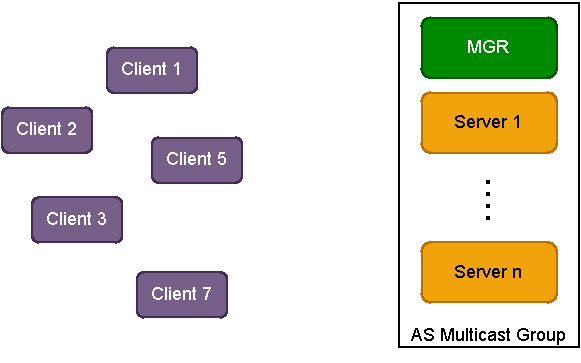
\includegraphics[scale=0.7]{graphics/DS_Architecture.pdf}
    \caption{Overview of the System Architecture}
    \label{fig:overview}
\end{figure}

An overview of the YACA system architecture can be found in \Cref{fig:overview}. YACA uses the client-server architecture, where clients are participants of a (single) global group chat and servers ensure that the chat history is replicated in a Byzantine fault-tolerant manner. In the following, we provide an overview of available administrator configuration, along with basic server and client functionality:

\subsection{Administrator Configuration}\label{sec:admin_config}
Before spawning system-components, the administrator is able to configure multiple components that remain unchanged during execution. This comprises the following settings:
\begin{itemize}
    \item Class D Internet address: An address, preferably within the Local Network Control Block (224.0.0.0 to 224.0.0.225), used by the servers for multicast traffic.
    \item 5 $\times$ UDP ports: Four predefined ports used by servers to consume new multicast messages (cf. \Cref{sec:overview}) and one predefined port for listening to broadcast messages.
    \item Timeout settings: Specification for different timeouts that might occur (e.g. heartbeats, polling-rates, timeouts for crash detection)
    \item Initial view: Specification of servers that are spawned at first startup. Each server is specified with an identifier, an IP address and listening-port, and a public key for digital signatures.\footnote{Note that the initial view is solely used by the servers as a base case, allowing new dynamically spawned servers the build a web of trust (cf. \Cref{sec:view_sync_comm}).}
\end{itemize}

\subsection{Server and Clients} \label{sec:overview}
On startup, the server is either part of the initial view, or joins the group by using the join-protocol described in \Cref{sec:view_sync_comm}. Most importantly, we use view-synchronous group communication, entailing that the new server builds a group view that is consistent with other correct servers' group views. Therefore, using a combination of view-synchronous group communication and digital signatures, we can realize closed group communication. As described in \Cref{sec:admin_config}, we use one multicast address where servers consume multicast messages over four UDP ports, each serving a different purpose:
\begin{enumerate}
    \item[i)] \textsf{C-Read}: R-multicast (cf. \Cref{sec:primitives}), where clients can query heartbeats and public keys of other clients.
    \item[ii)] \textsf{C-Write}: CO-R-multicast (cf. \Cref{sec:primitives}), where clients send new group chat messages to, or register to the service.
    \item[iii)] \textsf{S-Coordination}: CO-R-multicast, where \textit{exclusively} servers can perform the election algorithm and the phase-king algorithm.
    \item[iv)] \textsf{S-Announcements}: TO-R-multicast (cf. \Cref{sec:to_multicast}), where \textit{exclusively} servers announce elections and information about new servers is announced.
\end{enumerate}

\subsubsection{C-Read} 
Clients send new group chat messages to \textsf{C-Write}. To reduce the load of the servers, clients are only allowed to send messages, but not heartbeats or negative acknowledgements (cf. \Cref{sec:primitives}). Therefore, clients can periodically query servers' heartbeats via \textsf{C-Read}. Note that this mechanism can also be used by the clients to detect if there were omission failures. In response, the client receives heartbeats from multiple servers, which can then be contracted individually, via unicast, to retrieve the new group chat messages. Since the retrieved group chat messages contain vector timestamps, the client is able to recreate the chat history while respecting the happened-before relation.

The second important usage of \textsf{C-Read} is that a client can query public keys of other clients: Since clients sign every group chat message they sent, including the vector timestamp, malicious (i.e. Byzantine fault) servers cannot tamper with group chat messages, once the client knows about the corresponding public keys. To gain knowledge about these public signing keys, the client multicasts a query to the group of servers, collects their responses and performs a majority decision.

\subsubsection{C-Write}
On startup, clients create a random user ID and a digital signature key-pair. They then sent both via \textsf{C-Write} to the servers, which perform the phase-king algorithm (cf. \Cref{sec:consensus}) on the received data to ensure consensus.\footnote{This is required in case the client is malicious or there are multiple clients with the same user ID registering at the same time.} The servers respond afterward to notify the client whether the registration was successful. If necessary, the client retries the registration process.

Additionally, clients send their new group chat messages to \textsf{C-Write}. To ensure that other clients are able to rebuild the chat history while respecting the happened-before relation, new group messages contain the client's vector timestamps. Furthermore, the message, including the vector timestamp, is signed by the client to ensure that malicious servers cannot tamper with it.

\subsubsection{S-Coordination} 
Since TO-R-multicast used by \textsf{S-Announcements} has a non-negligible overhead, we use \textsf{S-Coordination} for messages that do not have to be total-ordered. There are mainly two applications for \textsf{S-Coordination}: When delivering a message via \textsf{S-Announcements}, we perform the phase-king algorithm on the delivered message contents to ensure that every correct server processes the same message.\footnote{This is required, since the original sender might send different messages, with the same sequence number, to different servers.} The second application is that \textsf{S-Coordination} can be used to perform elections, after delivering election announcements via \textsf{S-Announcements}. 

\subsubsection{S-Announcements}
As previously stated, \textsf{S-Announcements} is used to deliver election announcements and to announce newly joined servers. This ensures that join messages, as part of view-synchronous group communication, are delivered in the same order (cf. \Cref{sec:view_sync_comm}), and that every server has the same group-view when starting an election. 

Note that the phase-king algorithm also requires a consistent group-view, analogously to the election algorithm. Since the phase-king algorithm is also used for \textsf{C-Write}, while the max-phase-king algorithm is used to realize TO-R-multicast itself (cf. \Cref{sec:to_multicast}), we terminate all executions of the phase-king algorithm when \textsf{S-Announcements} delivers a join message.\footnote{To be more exact, we use hold-messages as described in \Cref{sec:view_sync_comm} to ensure that either every or no server terminates a phase-king execution.}

\subsection{Manager (MGR)}
We use leader election to determine a unique \textit{Manager (MGR)} of the servers. While the MGR behaves, for the most part, identical to other servers, he also listens to incoming broadcast messages. This is used by new servers to contact a server instance who is able to send messages to \textsf{S-Announcements}. This is required since servers only accept messages over \textsf{S-Announcement}, which were sent by other participants they already know.

For the sake of full transparency, we note that this utilization of the MGR is neither the most practical nor the most efficient one, and is instead mostly used to fulfill the formalities of the project requirements. For example, one disadvantage of this approach is other servers have to constantly monitor the MGR, by listening to broadcast themselves, in order to ensure that the \textit{non-triviality} guarantee of view-synchronous group communication is satisfied, since the MGR himself might be malicious.

\newpage
\section{Implementation Details}\label{sec:implementation}

\subsection{Primitives} \label{sec:primitives}

\subsubsection{Notation} We use $V$ to denote the (finite) set of server processes. To coincide with the notation of the lecture and \cite{ds_book}, we sometimes use $g$ do denote the server group.

\subsubsection{Messages}
In general, all messages inherit the base class \textsf{Message}, which includes fields for the message \textsf{Header}, \textsf{Content}, and \textsf{Metadata}. Furthermore, base functionalities include encoding and decoding the messages, using JSON. The message type is uniquely identified by the header, which tells the process how the message's content should be processed and which metadata is included. Examples for included metadata are digital signatures, sequence numbers, piggybacked acknowledgements, or nonces.

\subsubsection{Delivery Queues}
Another useful primitive is the FIFO delivery queue. Our general approach for processing incoming messages is to have one listening thread per listening port, which handles configuration messages (e.g. heartbeat messages, negative acknowledgements, or proposal messages for TO-multicast) and forwards only the relevant messages via a delivery queue to one or multiple worker threads. Therefore, we use locks to realize this in a thread-safe manner. Furthermore, we use semaphores to provide a blocking consume and a non-blocking produce operation. 

\subsubsection{Reliable Multicast (R-Multicast)}
In general, we implement R-multicast using a combination of reliable multicast over IP multicast, as described in \cite[p.~649]{ds_book}. Each process $p \in V$ manages a local sequence number $S_p$, which is initialized as zero and is atomically incremented each time $p$ sends a message, and a dictionary $R_g: V \rightarrow \mathbb{N}$, where $R_g(q)$ keeps track of $q$'s last delivered message sequence number (for each $q \in V$). When sending a message (via IP multicast), $p$ includes both $S_p$ and $R_g^p := \{(q, R_g(q)) | q \in V\}$ as metadata. Therefore, when a message $m$ is received with the attached sequence number $S$ by some process $q$, there are three possible cases:
\begin{enumerate}
    \item[i)] $S \leq R_g(q)$: $p$ already delivered $m$ and simply discards the duplicate 
    \item[ii)] $S = R_g(q)+1$: $p$ delivers $m$ and additionally stores it indefinitely
    \item[iii)] $S > R_g(q)+1$: $p$ detects that there are missing messages and places $m$ in a holdback-queue   
\end{enumerate}
Note that piggybacking $R_g^p$ to a message implicitly acts as an acknowledgement. As this only works if $p$ continuously sends messages, we periodically send heartbeat messages as well. 

If $p$ detects missing messages, by inspecting piggybacked acknowledgements of normal messages or heartbeat messages, it sends negative acknowledgements to the sender (which is not necessarily the original sender of the message). Since each message is digitally signed, we assume that messages forwarded in this manner cannot be manipulated by the forwarding process (which is an additional guarantee on top of the checksums used internally for IP multicast). After missing messages are delivered, $p$ checks its holdback-queue for messages that are now able to be delivered. 

Similar to the original protocol described in \cite[p.~649]{ds_book}, it is easy to see that above protocol satisfies the following properties:
\begin{itemize}
    \item \textit{Integrity:} Duplicates are detected by inspecting the attached sequence number. IP multicast uses checksums, and we use additional digital signatures to ensure that the received message is identical to the message signed by the sending process.
    \item \textit{Validity:} Trivially satisfied by the usage of IP multicast.
    \item \textit{Agreement:} Each process is able to detect that some process $q$ delivered $m$ by inspecting $R_g^q$ attached to the following messages. Since $q$ stores $m$ indefinitely, $p$ can request the missing message by sending negative acknowledgements.
\end{itemize}

\subsubsection{Causal-Ordered Reliable Multicast (CO-R-Multicast)}
The protocol above can now be extended to support causal ordering by using the strategy described in \cite[p.~657-658]{ds_book}: Each process manages a further holdback-queue and an additional vector stamp $R_g^{CO}: V \rightarrow \mathbb{N}$, where $R_g^{CO}(q)$ manages the last CO-R-delivered message sequence number of process $q$. When process $p$ R-delivers a message $m$ of sender $q$ with attached vector stamp $R$ and sequence number $S$, it places $m$ in the second holdback-queue until the contraints
\begin{enumerate}
    \item[i)] $R_g^{CO}(q) + 1 = S$, and 
    \item[ii)] $R_g^{CO}(q') \geq R(q')$ for each $q' \in V \backslash \{q\}$
\end{enumerate}
are satisfied. The proof of correctness is identical to the one given in \cite[p.~658]{ds_book}.

\subsection{Suspicion Protocol} \label{sec:suspicion}
When having malicious servers in our system it is advantageous to have a protocol that is able to suspend them, if inconsistent or incorrect behavior is detected. In this context, suspending a server means that no more incoming messages are accepted anymore, or to be more exact, no new message is accepted from the suspended server that was not already acknowledged by another server. This can easily be achieved by using digital signatures and only accepting messages that are gathered via negative acknowledgements. 

One straight-forward strategy to achieve an agreed suspension is to send \textit{suspect messages} to all other servers and suspend a server as soon as at least one suspect message has arrived. To avoid having a malicious server sending suspect messages for all servers and suspending them, we modify this protocol to allow for $f < n/3$ malicious servers (since we utilize the phase-king algorithm this limit is of course capped by $f < n/4$):
\begin{itemize}
    \item If detecting inconsistent or incorrect behavior (e.g. timeout on response), send a suspect message. The suspect message contains the suspected server identification and the reason why the server is suspected (e.g. ''proposal timeout on \textit{msg\_id}'' for the ISIS algorithm).
    \item If a server gathers more than $f$ suspect messages for the same server and the same reason, he sends a suspect message himself if he did not already send one.
    \item If a server gathers at least $n-f$ suspect messages, the server is suspended (cf. \Cref{sec:view_sync_comm}).
\end{itemize}
For the guarantees of the above protocol, it is easy to see that if a server gathers $n-f$ suspect messages, he can be sure that all other correct processes gather at least $n-2f > f$ (for $f < n/3$) suspect messages of the same kind. Thus, eventually, every correct process eventually sends a suspect message. On the other hand, if a server receives at least $f$ suspect messages, he can be sure that at least one correct (or honest) server is suspecting the accused server.

\subsection{(Max-)Phase-King Algorithm}\label{sec:consensus}
To provide resilience against Byzantine faults (with $f < n/4$), we use the Phase-King Algorithm \cite{phaseking} and our Max-Phase-King Algorithm (cf. \Cref{appendix:maxphaseking}). We use CO-R-multicast which separates different phases and their rounds more elegantly, i.e., the phase-king message of round 2 is delivered after all round 1 messages are delivered. 

Another important aspect is that each participant agrees on the same phase-king. The same problem occurs for our election mechanism and is solved by utilizing view-synchronous group communication (cf. \Cref{sec:view_sync_comm}). This allows us to manage a consistent list of unsuspended server IDs across all server instances, yielding that the $i$th entry of the list is selected as the phase-king of phase $i$. 

Furthermore, we use the suspicion protocol described in \Cref{sec:suspicion}. This ensures that processes are not stuck waiting for messages in round 1, when gathering $N$ messages, or in round 2, when receiving the tiebreaker value of the phase-king. In case the phase-king is suspended, the next phase-king simply takes over (avoiding the need to choose the default value as the tiebreaker).

\subsection{Election} \label{sec:election}
It is easy to see that ring-based election algorithms are prone to a wide range of failures, making them unappealing. Analogously, the bully algorithm \cite[p.~644-645]{ds_book} does not provide resilience against Byzantine failures, e.g., an arbitrary processes might immediately send \textit{coordinator} messages, causing an inconsistent result for the election. Therefore, we realize a Byzantine fault-tolerant election algorithm by utilizing more powerful building blocks: The phase-king algorithm (cf. \Cref{sec:consensus}) and group-synchronous group communication (cf. \Cref{sec:view_sync_comm}).

\lstset{
    basicstyle=\ttfamily,
    breaklines=true,
    language=C++,
    escapeinside={\%(}{\%)},
    commentstyle=\color{darkgreen},
    frame=single,
    keywords={def, function, begin, end, for, do, done, broadcast, await, if, then, else, receive, pass, output, in, return},
    keywordstyle=\bfseries\color{blue},
    numbers=left,
}
\begin{lstlisting}
function Election(servers : list) for %($p_i \in V$%) begin 
    elected = %($\bot$%) 
    for server in servers do
        init_value : %($\{0, 1\}$%) 
        if is_reachable(server) then 
            init_value %($\leftarrow$%) 1 
        else 
            init_value %($\leftarrow$%) 0 

        result %($\leftarrow$%) phase_king(init_value)
        if result == 1 then 
            elected %($\leftarrow$%) server
            return
    done
end
\end{lstlisting}
It is easy to see that above election algorithm satisfies both \textit{safety} and \textit{liveness} requirements. We note that we use the definitions of the lecture, which slightly deviate from the ones given in \cite[p.~642]{ds_book}, and adopt the notation: Let $V$ be the set of processes, and $V_g \subseteq V$ the set of correct processes. Each process $p_i \in V$ has a variable $elected_i$, which is either undefined (i.e. $elected_i = \bot$) or contains the identifier of the elected process. Safety and liveness are then defined as:
\begin{enumerate}
    \item[i)] \textit{Safety:} $\forall p_i \in V_g: elected_i = \bot \text{ or } \left(\forall p_j \in V_g: elected_i = elected_j\right)$
    \item[ii)] \textit{Liveness:} Every correct process $p_i \in V_g$ eventually sets $elected_i \neq \bot$
\end{enumerate}
For safety, it is easy to see that if $p_i \in V_g$ sets $elected_i = p_k \neq \bot$ for some $p_k \in V$, the result of the phase-king algorithm is $1$ for $p_k$. Therefore, every other correct process $p_j$ has the same result for the phase-king algorithm,\footnote{The proof of this guarantee is similar to the one presented in \Cref{theorem:maxpk}} resulting in $elected_j = p_k$. Note that this implicitly requires that every process shares the same input list \texttt{servers}, which we guarantee be using view-synchronous group communication.

For liveness, we use the fact that the phase-king algorithm requires $f < n/4$. Therefore, the for-loop in line $(3)$ eventually selects a correct server $p_k$, i.e., after at most $f+1$ iterations. By assumption, the $p_k$ responds to the incoming ping-messages of other servers, resulting in $init\_value_i = 1$ for every $p_i \in V_g$. Since $|V_g| = n-f > n/2 + f$, the correct processes always use the majority value in round 2 of every phase in the phase-king algorithm. Therefore, the result of the phase-king algorithm is $1$ as well and $elected_i$ is set to $p_k \neq \bot$.\footnote{A similar argument provides an even stronger guarantee than safety, where the elected process appears as ''not-crashed'' to at least one correct process. }

\subsection{Total-Ordered Reliable Multicast (TO-R-Multicast)} \label{sec:to_multicast}
We build TO-R-multicast on top of CO-R-multicast using the ISIS algorithm described in \cite[p.~655-656]{ds_book}. We use CO-R-multicast instead of R-multicast for the following three reasons:
\begin{enumerate}
    \item[i)] Proposal messages are delivered after the original message
    \item[ii)] To implement the suspicion protocol (cf. \Cref{sec:suspicion}) and to suspend processes (cf. \Cref{sec:view_sync_comm})
    \item[iii)] To perform the max-phase-king algorithm (cf. \Cref{appendix:maxphaseking}) on the agreed sequence numbers   
\end{enumerate}
We note that this, however, does not guarantee that the total-ordered messages satisfy causal-ordering as well.

Each server $p$ maintains variables $P_g^p$ and $A_g^p$. Upon sending a message via TO-R-multicast, the sender adds a randomly generated message ID and CO-R-multicasts it. When a server CO-R-delivers such a message, he responds with a proposal $P_g^p = max(A_g^p, P_g^p)+1$ for the message's sequence number. This is also done via CO-R-multicast, as opposed to unicast \cite[p.~655-656]{ds_book}. This allows us to use the max-phase-king algorithm directly as described in \Cref{appendix:maxphaseking}. While waiting for all proposals to arrive, the message is stored in a sorted hold-back queue. For sorting, we use the tuples $(seqno, msg\_id)$, where $seqno$ is the largest received proposal and
\begin{align*}
    (seqno1, msg\_id1) < (seqno2, msg\_id2) \iff (seqno1 < seqno2 \text{ or } \\
    (seqno1 = seqno2 \text{ and } msg\_id1 < msg\_id2)).
\end{align*}
When the max-phase-king algorithm completed its execution for a message ($v_{init}$ is the largest gathered proposal), its respective entry in the hold-back queue is marked as \textit{ready-to-deliver}. A message is moved from the hold-back queue to the FIFO-ordered delivery queue if and only if it is marked as ready-to-deliver, and it is first in the hold-back queue. As before, we use the suspicion protocol (cf. \Cref{sec:suspicion}) if processes experience timeouts while waiting for proposals.

For the proof of correctness, consider two correct processes $p_i$ and $p_j$, where $p_i$ delivers a message $msg_1$ before $msg_2$. Since we use a FIFO-ordered delivery queue, $msg_1$ is added to the queue before $msg_2$. Consider the time-point, where $p_i$ adds $msg_1$ to the delivery queue. There are two cases to inspect:
\begin{enumerate}
    \item[i)] \textit{$p_i$ did not propose a sequence number for $msg_2$ yet:} Let $S_1$ be the assigned sequence number of $msg_1$ (after the max-phase-king algorithm). Then, we have $S_1 \leq A_g^{p_i}$ and $p_i$ proposes some sequence number $P_2$ for $msg_2$ with $P_2 = max(A_g^{p_i}, P_g^{p_i})+1 > A_g^{p_i} \geq S_1$. Since $p_i$ and $p_j$ are correct, $p_j$ shares the same value for $S_1$ and the max-phase-king algorithm further ensures that the final sequence number $S_2$ for $msg_2$ is larger than $S_1$ (cf. \Cref{theorem:maxpk}). Therefore, $p_j$ also delivers $msg_1$ before $msg_2$.
    \item[ii)] \textit{$p_i$ did already propose a sequence number for $msg_2$:} Using the same notation as above, we know that $msg_1$ is first in the ordered hold-back queue, before it is appended to the delivery queue. Let $P_2$ be the largest proposal for $msg_2$ that was received by $p_i$ yet. Since $(S_1, id(msg_1)) < (P_2, id(msg_2))$, we either have $S_1 < P_2$, or $S_1 = P_2$ and $id(msg_1) < id(msg_2)$. In the first case, the max-phase-king algorithm is later executed for $msg_2$ with $v_{init}^i \geq P_2$, resulting in an output $S_2 \geq P_2 > S_1$ (cf. \Cref{theorem:maxpk}). In the second case, we have the same argument resulting in $S_2 \geq P_2 \geq S_1$, where $id(msg_1) < id(msg_2)$ again decides that $msg_1$ is delivered before $msg_2$. Therefore, it can be seen that $p_j$ delivers $msg_1$ before $msg_2$ as well.
\end{enumerate}


\subsection{View-Synchronous Group Communication} \label{sec:view_sync_comm}
In view-synchronous group communication, new processes can join and participants can be suspended. 
\begin{enumerate}
    \item[i)] \textit{Suspension:} We extend the suspicion protocol described in \Cref{sec:suspicion}. Furthermore, our servers listen to multiple multicast instances (i.e. one for TO-R-multicast and two for CO-R-multicast), which is also considered in the following: 
    \begin{itemize}
        \item If a server $p$ detects inconsistent or incorrect behavior, or receives more than $f$ suspect messages (cf. \Cref{sec:suspicion}), $p$ sends a suspect message via each multicast instance.
        \item If $p$ gathers at least $n-f$ suspect messages for servers $q_1, \ldots, q_k$, he sends \textit{hold-messages} $h_1, \ldots, h_k$, where $h_i$ contains information about $q_i$, and stops sending new messages, except for additional suspect and hold messages. He waits for the corresponding hold messages for $q_1, \ldots, q_k$ of all other servers. If a server $q$ does not send a hold message within a timeout interval, $p$ send a suspect message for $q$ as well. 
        \item Let $q_1, \ldots, q_k, \ldots, q_{k+l}$ be the enqueued servers for suspension (i.e. $p$ received more than $n-f$ suspect messages for each $q_i$). After $p$ received $n-k-l$ different hold messages for each $q_i$ on each multicast instance, he suspends every $q_i$ and continues normal operation.
    \end{itemize} 
    \item[ii)] \textit{Join:} On first startup, the administrator can configure an \textit{initial view}, where multiple server instances are spawned and share a consistent group view. This initial view contains information about the server ID, IP address and listening-port for unicast messages, and a public key for digital signatures. Servers that are spawned afterwards also know the initial view, but yet have to learn about the servers that joined afterwards (e.g. all servers included in the initial view might already have crashed). 
    \begin{itemize}
        \item When a new server $p$ wants to join the group of servers, he sends a request to the MGR (via broadcast) containing $p$'s ID, IP address and listening-port, and a public key for digital signatures.
        \item When the MGR receives such a request he validates that $p$'s ID is unique, encapsulates the request in a signed \textit{join-message}, and forwards it via TO-R-multicast. Note that signing the join-message is crucial as other servers only accept messages of participants. Furthermore, note that other servers can validate the correct behavior of the MGR by listening to broadcast as well. 
        \item When a participant $q$ delivers the join-message of $p$, $q$ sends an acknowledgement to $p$ adds the encapsulated information to its group-view, but marks $p$ as still \textit{inactive}. Furthermore, $q$ sends a hold-message on each multicast instance (identical to $i)$). 
        \item When $p$ receives the first acknowledgement, he is now able to send negative acknowledgements and is therefore able to consume the messages of every multicast instance. When reaching the corresponding hold-messages (containing $p$'s ID), $p$ sends a \textit{commence-message} to tell other participants to resume normal operation.\footnote{Most importantly, this mechanism allows $p$ to build its own consistent group view: Using an inductive argument, $p$ starts with the initial view (i.e. the base case) and is able to verify the signatures of the initial processes. Any process $q$ that joined thereafter must have used the same protocol as $p$, which allows $p$ to validate that $q$ was indeed added to the group-view. This way, $p$ also learns of $q$'s public key, which enables $p$ to build a web of trust and validate new messages of $q$. Analogously, $p$ collects suspect messages and suspends processes if necessary. By simulating previous elections and phase-king executions, $p$ is then able to rebuild the consistent state and group-view in a Byzantine fault-tolerant manner. }
        \item When $q$ receives a commence-message from $p$ on each multicast instance, he marks $p$ as \textit{active} and continues normal operation. Note that the first message of $p$ is expected to be a commence-message. Otherwise, $q$ simply sends a suspect message for $p$. Similarly, $q$ is able to set a timeout interval.
    \end{itemize} 
\end{enumerate}
When considering view-Synchronous group communication as defined in \cite[p. ~772-773]{ds_book}, we need to argue that the guarantees \textit{order, integrity, non-triviality, agreement, and validity} are satisfied. Due to space restrictions, we include the proof of correctness in \Cref{appendix:view_sync_comm}.

\section{Conclusion and Discussion} \label{sec:conclusion}

%
% ---- Bibliography ----
%
\bibliographystyle{plain} % We choose the "plain" reference style
\bibliography{bibtex}

\newpage 
\appendix
\section{Appendix}\label{appendix}
\subsection{Max-Phase-King Algorithm}\label{appendix:maxphaseking}
\lstset{
    basicstyle=\ttfamily,
    breaklines=true,
    language=C++,
    escapeinside={\%(}{\%)},
    commentstyle=\color{darkgreen},
    frame=single,
    keywords={def, function, begin, end, for, do, done, broadcast, await, if, then, else, receive, pass, output},
    keywordstyle=\bfseries\color{blue},
    numbers=left,
}
\begin{lstlisting}
function MaxPhaseKing(%($v_{init}$%): int, %($f$%): int) for %($p_i \in V$%) begin 
    // Preparation
    broadcast %($v_{init}$%) to all processes
    await value %($v_j$%) from each process %($p_j \in V$%)
    %($\tilde{v}$%) %($\leftarrow$%) %($max\{v_j \mid p_j \in V\}$%)
    %($v$%) %($\leftarrow$%) %($\tilde{v}$%)

    for %($phase$%) = %($1,\ldots,f+1$%) do
        // Round 1
        broadcast %($v$%) to all processes
        await value %($v_j$%) from each process %($p_j \in V$%)
        %($mode$%) %($\leftarrow$%) mode of the %($v_j$'s%)
        %($mult$%) %($\leftarrow$%) number of times that %($mode$%) occurs 
        %($median$%) %($\leftarrow$%) median of the %($v_j$'s%)

        // Round 2
        if %($i = phase$%) then 
            broadcast %($\lceil median \rceil$%) to all processes 
        receive %($tiebreaker$%) from %($p_{phase}$%)
        if %($mult > |V|/2 + f$%) then 
            %($v$%) %($\leftarrow$%) %($mode$%)
        else if %($|\{v_j \mid v_j \leq tiebreaker\}| > f$%)
            %($v$%) %($\leftarrow$%) %($tiebreaker$%)
    done

    output %($v$%)
end
\end{lstlisting}

\subsubsection{Notation} As before, we use $V$ to denote the set of all processes. Let $n := |V|$ and $f < \lceil n/4 \rceil$ be the number of malicious processes. We denote $V_g \subseteq V$ as the set of correct processes and use the notation $v^{(p, k)}$ to denote the value of $v$ for process $p$ in phase $k$ ($k=0$ is used for the preparation phase). If the variable does not change with different phases, we omit $k$.

\subsubsection{Proof of Correctness} Our main goal is to show that all correct processes output the same value $v$ and that $v \geq v_{init}^{(p)}$ for all $p \in V_g$.

\begin{lemma}\label{lemma:maxpk1}
    Let $p_i$ be the phase-king. If $p_i$ is correct then $|\{v_j^{(p_k,i)} \mid v_j^{(p_k,i)} \leq tiebreaker^{(p_k,i)}\}| > f$ for all correct processes $p_k \in V_g$.
\end{lemma}

\begin{proof}
    If $p_i$ is correct, he gathers $\{v_j^{(p_i,i)} \mid p_j \in V\}$. After rewriting these values as 
    \begin{align*}
        v_{(1)} \leq v_{(2)} \leq \ldots \leq v_{(n)},
    \end{align*}
    the median is computed as $median = v_{(\frac{n+1}{2})}$ if $n$ is odd, or $median = (v_{(\frac{n}{2})} + v_{(\frac{n}{2}+1)})/2$ if $n$ is even. In both cases we have that 
    \begin{align*}
        |\{v_j^{(p_i,i)} \mid v_j^{(p_i,i)} \leq \lceil median \rceil\}| \geq \left\lceil \frac{n}{2} \right\rceil,
    \end{align*} 
    which in turn yields:
    \begin{align*}
        |\{v_j^{(p_k,i)} \mid v_j^{(p_k,i)} \leq tiebreaker^{(p_k,i)}\}| &\geq |\{v_j^{(p_i,i)} \mid v_j^{(p_i,i)} \leq \lceil median \rceil\}| - f \\
        &\geq \left\lceil \frac{n}{2} \right\rceil - f \\
        &> \left\lceil \frac{n}{2} \right\rceil - \left\lceil \frac{n}{4} \right\rceil  \\
        &\geq \left\lceil \frac{n}{4} \right\rceil - 1 \qquad \geq \; f
    \end{align*} \qed
\end{proof}

\begin{lemma}\label{lemma:maxpk2}
    Let $p_i$ be the phase-king. If $p_i$ is correct, then all correct processes share the same value for $v$ after the current phase. 
\end{lemma}
\begin{proof}
    Let $p_j$ and $p_k$ be arbitrary correct processes. Due to \Cref{lemma:maxpk1}, $v$ is updated with the $mode$ or the $tiebreaker$ value. Therefore, there are three cases to consider:
    \begin{enumerate}
        \item[i)] $p_j$ and $p_k$ use their $mode$ value: Then, $p_j$ received $mode^{(p_j,i)}$ more than $n/2+f$ times, which implies that $p_k$ also received $mode^{(p_j,i)}$ more than $n/2$ times. Therefore, there is no other possibility than $mode^{(p_k,i)} = mode^{(p_j,i)}$.
        \item[ii)] $p_j$ uses its $mode$ value and $p_k$ uses the $tiebreaker$ value: As before, $p_j$ received $mode^{(p_j,i)}$ more than $n/2+f$ times, which implies that the phase-king $p_i$ also received $mode^{(p_j,i)}$ more than $n/2$ times. Therefore, we have $median^{(p_i,i)} = mode^{(p_j,i)} \in \mathbb{N}$, which is then received by $p_k$ as the $tiebreaker$.
        \item[iii)] $p_j$ and $p_k$ use the $tiebreaker$ value: As $p_i$ is assumed to be correct, both receive the same $tiebreaker$ value. 
    \end{enumerate} \qed
\end{proof}

\begin{lemma}\label{lemma:maxpk3}
    Let $1 \leq i \leq f+1$ be a phase with a correct phase-king. Then, the following holds true:
    \begin{align*}
        \forall p_j, p_k \in V_g \forall phase \in \{i, \ldots, f+1\}: v^{(p_j, phase)} = v^{(p_k, phase)}
    \end{align*}
    That is, once there was a correct phase-king, all correct processes continue to share the same value for $v$ afterwards. 
\end{lemma}
\begin{proof}
    \Cref{lemma:maxpk2} handles the case of $phase = i$. Afterwards, all correct processes broadcast the same value of $v$, which implies that $mult^{(p_j, phase)} \geq n-f > n/2+f$ is satisfied for all $p_j \in V_g$ and $i < phase \leq f+1$. Using the same argument as $i)$ in the proof of \Cref{lemma:maxpk2}, it is easy to see that the statement holds true. \qed
\end{proof}

\begin{lemma}\label{lemma:maxpk4}
    The following statement holds true:
    \begin{align*}
        \forall p_j, p_k \in V_g \forall phase \in \{0, \ldots, f+1\}: v^{(p_j, phase)} \geq v_{init}^{(p_k)}
    \end{align*}
    That is, the value of $v$ for a correct process $p_j$ is always larger than the initial values of all correct processes. 
\end{lemma}
\begin{proof}
    We use an inductive argument to prove this statement. For $phase = 0$, $v^{(p_j,0)}$ is initialized in line 6. As all correct processes $p_k$ broadcast their initial value $v_{init}^{(p_k)}$ the statement is trivially satisfied. 

    For $phase > 0$, $v^{(p_j,phase)}$ there are three cases to consider:
    \begin{enumerate}
        \item[i)] $v^{(p_j,phase)}$ is not updated, i.e., $v^{(p_j,phase)} = v^{(p_j,phase-1)}$: By the induction hypothesis, the statement holds true. 
        \item[ii)] $v^{(p_j,phase)}$ is updated in line 21. Then $mult^{(p_j, phase)}  > n/2+f$ which implies that at least one correct process $p_l$ sent $mode^{(p_j, phase)}$ at the beginning of the phase. Using the induction hypothesis, we have:
        \begin{align*}
            v^{(p_j,phase)} = mode^{(p_j, phase)} = v^{(p_l,phase-1)} \geq v_{init}^{(p_k)}, \quad \forall p_k \in V_g
        \end{align*} 
        \item[iii)] $v^{(p_j,phase)}$ is updated in line 23. Let
        \begin{align*}
            C = \{v_k^{(p_j,phase)} \mid v_k^{(p_j,phase)} \leq tiebreaker^{(p_j,phase)}\},
        \end{align*}
        then the condition in line 22 states $|C| > f$. Therefore, there exists at least one correct process $p_l$ with $v_l^{(p_j,phase)} \in C$. This yields:
        \begin{align*}
            v^{(p_j,phase)} = tiebreaker^{(p_j,phase)} \geq v_l^{(p_j,phase)} = v^{(p_l,phase-1)} \geq v_{init}^{(p_k)},
        \end{align*}
        for all $p_k \in V_g$.
    \end{enumerate} \qed
\end{proof}

\begin{theorem}\label{theorem:maxpk}
    Each correct process $p_j$ that executes the max-phase-king algorithm outputs $v^{(p_j, f+1)}$ that satisfies
    \begin{enumerate}
        \item[i)] $\forall p_k \in V_g: v^{(p_j, f+1)} = v^{(p_k, f+1)}$, and 
        \item[ii)] $\forall p_k \in V_g: v^{(p_j, f+1)} \geq v_{init}^{(p_k)}$.
    \end{enumerate}
\end{theorem}
\begin{proof}
    \Cref{lemma:maxpk3} proves statement $i)$ and \Cref{lemma:maxpk4} proves statement $ii)$. \qed
\end{proof}

\subsection{View-Synchronous Group Communication} \label{appendix:view_sync_comm}
For formal reasons, we consider a sequence of views 
\begin{align*}
    v_0(g), v_1(g), \ldots, v_i(g), \ldots,
\end{align*}
where $v_0(g) = (p_1, \ldots, p_l)$ is the initial view specified by the administrator and $v_i(g)$ is of the following form:
\begin{equation}
    \begin{aligned}\label{eq:view}
        v_i(g) &= v_{i-1}(g) + (p) - (q_1, \ldots, q_l), &&\text{or}\\
        v_i(g) &= v_{i-1}(g) - (q_1, \ldots, q_l), &&\forall j \in \{1, \ldots, l\}: q_j \in v_{i-1}(g).
    \end{aligned}
\end{equation}
That is, a view delivery includes at most one joining process and potentially multiple suspended processes. 

In the following, we show that our implementation described in \Cref{sec:view_sync_comm} satisfies the guarantees described in \cite[p.~772-773]{ds_book}. As before, we assume a maximum of $f < n/4$ incorrect processes. Therefore, we restrict the \textit{non-triviality} guarantee to group partitions, where one partition contains more than $2n/3$ processes and demand only that this partition continues to function.
\begin{enumerate}
    \item[i)] \textit{Order:} Let $p$ and $q$ be correct processes that deliver the views $v(g)$ and $v'(g)$. If $p$ delivers view $v(g)$ before $v'(g)$, there exists $i, j \in \mathbb{N}_{\geq 1}$ with $v(g) = v_i(g)$ and $v'(g) = v_{i+j}$. Due to the total-ordering of join-messages, we can also assume that $v_i(g), \ldots, v_{i+j}(g)$ are of the second form, as described in \Cref{eq:view} (otherwise, \textit{Order} is trivially satisfied). Before $p$ delivers $v(g)$, $p$ collects hold-messages from all processes that are not enqueued for suspension. In particular, $p$ received corresponding hold messages from $q$, which entails that $q$ was also collecting suspect messages for the same processes as $p$. Using the guarantees of our suspicion protocol (cf. \Cref{sec:suspicion}), it is easy to see that $p$ and $q$ eventually suspend the same processes. Therefore, $q$ also delivers $v(g)$ before $v'(g)$.
    \item[ii)] \textit{Agreement:} In addition to the \textit{Order} guarantee, \textit{Agreement} also demands that every correct process delivers the same messages in every view. This is achieved by using hold-messages as described in \Cref{sec:view_sync_comm} in combination with CO-R-multicast. 
    \item[iii)] \textit{Integrity:} If a correct process $p$ delivers view $v(g)$, then $p$ is not suspended since it would have terminated otherwise. Therefore, $p \in v(g)$ holds true. Furthermore, if $p$ delivers a message $m$, then the guarantees of CO-R-multicast entail that $p$ will not deliver $m$ again. Finally, the usage of hold-messages ensures that $sender(m)$ is in the view in which $p$ delivers $m$.
    \item[iv)] \textit{Non-triviality:} If a correct process $q$ joins the group, it contacts the MGR via broadcast to forward the join-message to all participants via TO-R-multicast. As other participants also listen to broadcast, they can detect if the MGR does not forward join requests and send suspect messages. Therefore, we can assume that the join-message of $q$ is eventually delivered by every participant via TO-R-multicast. By construction, $q$ then consumes the messages of every multicast instance and is afterwards considered as an active participant.
    
    Analogously, correct processes eventually detect group partitions via timeouts and send suspect messages. Using the guarantees of our suspicion protocol (cf. \Cref{sec:suspicion}), the processes of other partitions are eventually suspended, as long as the own partition contains more than $2n/3$ processes. 
    \item[v)] \textit{Validity:} Because of the validity guarantee of CO-R-multicast, correct processes always deliver the messages that they send. If the system fails to deliver a message to any process $q$, other correct processes will notice a timeout when waiting for the hold-messages of $q$ before delivering a new view (if the timeout is not noticed before). Since this timeout is detected by $n-f$ correct processes, $q$ will be suspended and excluded from the next view. 
\end{enumerate}

\end{document}
